\documentclass[tikz,border=10pt]{standalone}
\usepackage{pgfplots}
\pgfplotsset{compat=1.18}
\usetikzlibrary{arrows.meta, calc}

\begin{document}
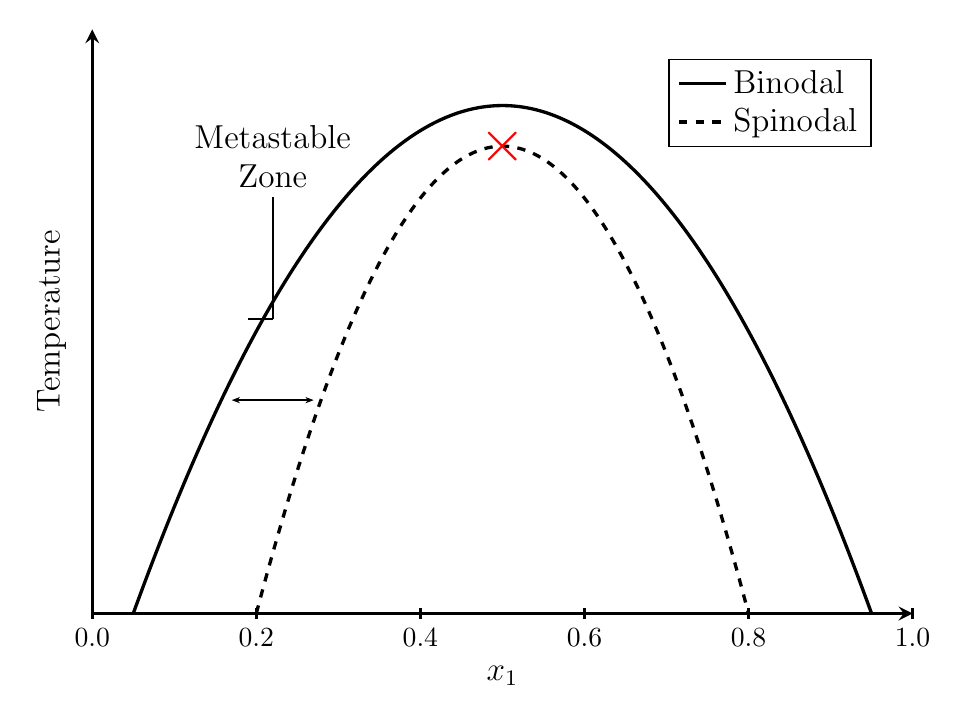
\begin{tikzpicture}
\begin{axis}[
    width=12cm,
    height=9cm,
    axis lines=left,
    xlabel={$x_1$},
    ylabel={Temperature},
    xlabel style={font=\large},
    ylabel style={font=\large, at={(axis description cs:-0.02,0.5)}},
    axis line style={very thick},
    xmin=0, xmax=1,
    ymin=0, ymax=1.15,
    xtick={0.0, 0.2, 0.4, 0.6, 0.8, 1.0},
    xticklabels={0.0, 0.2, 0.4, 0.6, 0.8, 1.0},
    ytick=\empty,
    clip=false,
    legend style={
        at={(0.95,0.95)},
        anchor=north east,
        draw=black,
        fill=white,
        font=\large,
        cells={anchor=west},
        legend cell align=left,
    },
    every tick/.style={very thick},
]

% --- Binodal curve (solid) ---
% Parabolic dome: T = A*(x - x_L)*(x_R - x) where x_L ~ 0.05, x_R ~ 0.95
% Max at x = 0.5: A*(0.45)*(0.45) = A*0.2025 = 1.0 => A = 4.938
\addplot[
    black,
    very thick,
    solid,
    domain=0.05:0.95,
    samples=200,
] {4.938*(x - 0.05)*(0.95 - x)};
\addlegendentry{Binodal}

% --- Spinodal curve (dashed) ---
% Narrower dome: T = B*(x - 0.2)*(0.8 - x), max at 0.5: B*0.09 = 0.92 => B = 10.222
\addplot[
    black,
    very thick,
    dashed,
    domain=0.2:0.8,
    samples=200,
] {10.222*(x - 0.2)*(0.8 - x)};
\addlegendentry{Spinodal}

% --- Red X at spinodal maximum (x=0.5, T=0.92) ---
\node[red, font=\Large\bfseries, scale=1.5] at (axis cs:0.5, 0.92) {$\times$};

% --- Metastable Zone annotation ---
% Label with arrow pointing to the gap between binodal and spinodal on left side
\node[font=\large, align=center, anchor=south] at (axis cs:0.22, 0.82) {Metastable\\Zone};
% Arrow from label down to the gap region
\draw[thick] (axis cs:0.22, 0.82) -- (axis cs:0.22, 0.58);
\draw[thick] (axis cs:0.22, 0.58) -- (axis cs:0.19, 0.58);
% Small horizontal double arrow showing the gap
\draw[thick, {Stealth[length=3pt]}-{Stealth[length=3pt]}] (axis cs:0.17, 0.42) -- (axis cs:0.27, 0.42);

\end{axis}
\end{tikzpicture}
\end{document}
